\documentclass[
	,footlinenumber
	,navline=true
	,footlineauthor
	,ngerman
	]{beamer}

\definecolor{coolgray}{rgb}{0.90625,0.8828125,0.8359375}
\definecolor{BurntOrange}{rgb}{1,0.5,0}
\definecolor{Brown}{HTML}{C17D11}
\definecolor{SeaGreen}{HTML}{2e8b57}

\usepackage{babel}
\usepackage[utf8]{inputenc}
\usepackage[T1]{fontenc}
\usepackage{lipsum}
\usepackage{ifthen}
\usepackage{multirow}
\usepackage{tikz}
\usepackage{color}
\usepackage{soulutf8}
\usepackage{marvosym}
\usepackage{wasysym}
\usepackage{textcomp}
\usepackage{multicol}
\usepackage{etex}	%wegen mehr dimensions..
\usepackage{filecontents}
\usepackage{appendixnumberbeamer}
\usepackage{fancyvrb}

\usepackage{pgfpages}
%\setbeameroption{show notes on second screen=right}
\setbeamertemplate{note page}{%
	\insertnote%
}

\fvset{fontsize=\small}
\usepackage{listings}
\lstset{
  language=TeX,
  morekeywords={begin,documentclass,usepackage,section,subsection,subsubsection}, 
%Umlaute in listings 
  literate=%
	{Ö}{{\"O}}1
	{Ä}{{\"A}}1
	{Ü}{{\"U}}1
	{ß}{{\ss}}1
	{ü}{{\"u}}1
	{ä}{{\"a}}1
	{ö}{{\"o}}1,
	breaklines=true,
	}

	

\newcommand{\zwischenUebersicht}
{
   \begin{frame}
        \frametitle{\"Ubersicht}
	\note{
        \tableofcontents[ 
    		currentsubsection, 
%		hideothersections, 
		hideothersubsections,
   		sectionstyle=show/hide, 
%		sectionstyle=show/shaded, 
%		subsectionstyle=show/hide, 
		] 
	}
%	\tableofcontents[ 
%    		currentsubsection, 
%%		hideothersections, 
%		hideothersubsections,
%%   		sectionstyle=show/hide, 
%		sectionstyle=show/shaded, 
%		subsectionstyle=hide, 
%		] 
	\begin{columns}[t]
        \begin{column}{.5\textwidth}
            \tableofcontents[subsectionstyle=show,hideothersubsections,sectionstyle=show/shaded,sections={1-3}]
        \end{column}
        \begin{column}{.5\textwidth}
            \tableofcontents[subsectionstyle=show,hideothersubsections,sectionstyle=show/shaded,sections={4-6}]
        \end{column}
    \end{columns}
   \end{frame}
}


%Easy Quoteblock
%Use: \quoteblock{Quoute Adii as manimus.}{Wurstlet}
\newcommand{\quoteblock}[2]
{
\begin{block}{}
\begin{quote}
    ``#1''
  \end{quote}
  \vskip3mm
  \hspace*\fill{\small--- #2} 
\end{block}
}

\newcommand{\miniblock}[2]
{
\hspace*{.1\linewidth}\begin{minipage}{.8\linewidth}
    \begin{block}{#1}
      #2
    \end{block}
    \end{minipage}
}

\usepackage{tikz}
\usetikzlibrary{shapes,snakes,arrows}
\usetikzlibrary{positioning}
\usetikzlibrary{arrows}
\usepackage{pgfplots}
\usetikzlibrary{calc,fadings,decorations.pathreplacing}

\usepackage{amsmath,amssymb}
\usepackage{array}
\usepackage{mathrsfs}
\usepackage{listings}

\usepackage{boxedminipage}

\graphicspath{{../pictures/}}

\tikzstyle{mybox} = [draw=red, fill=coolgray, very thick,
    rectangle, rounded corners, inner sep=5pt, inner ysep=10pt,
	text width=.9\textwidth]
\tikzstyle{fancytitle} = [fill=red, text=white, rounded corners]

\DeclareMathOperator{\ArcSin}{ArcSin}
\DeclareMathOperator{\ArcCos}{arc cos}

\mode<presentation>
{  
	\usetheme[headlinetitle={geht nicht, siehe outer theme z. 166}]{Bremen}
	\fbnum{03}
	\fbname{RY-AVS}
	\institutelogo{z. 159 im outertheme.}
	\title{geht nicht, siehe outer theme z. 166}
}

\usepackage[scaled=.90]{helvet}
\renewcommand\ttdefault{txtt}
\usefonttheme[onlymath]{serif}

\title{Protective Avionics Flash File System\\PAFFS}
\author[Pascal.Pieper@dlr.de]{Pascal Pieper}

\date{\today}


\begin{document}
\setbeamertemplate{caption}{\raggedright\insertcaption\par} %Kein ``Abbildung: `` vor captions


\begin{frame}
\titlepage
\end{frame}
\begin{frame}[t]{Table of contents}
    \begin{columns}[t]
        \begin{column}{.5\textwidth}
            \tableofcontents[hideothersubsections,sections={1-3}]
        \end{column}
        \begin{column}{.5\textwidth}
            \tableofcontents[hideothersubsections,sections={4-6}]
        \end{column}
    \end{columns}
\note {
    \begin{multicols}{2}
    \tableofcontents
    \end{multicols}
    
    }
\end{frame}


\section{Introduction}
\zwischenUebersicht
\subsection{Overview}
\begin{frame}{Overview}
\begin{block}{Computer guided spaceflight}
\begin{itemize}
\item Consisting of many subparts
\begin{itemize}
\item Focus of this work is mass storage
\end{itemize}
\item Experiment data (payload) 
\item Instructions 
\item Program images
\begin{itemize}
\item[$\rightarrow$] Many applications for long term memory
\end{itemize}
\end{itemize}
\end{block}
\end{frame}

\begin{frame}{Overview}
\begin{block}{Negative influences on memory}
\begin{itemize}
\item Vibrations
\item Radiation
\item Rapid temperature changes
\item Hard heat dissipation
\end{itemize}
\end{block}
\end{frame}

\begin{frame}{Overview}
\begin{block}{Solution}
\begin{itemize}
\item Radiation tolerant and robust memories
	\begin{itemize}
	\item<alert@1-> High cost
	\end{itemize}
\end{itemize}
\end{block}
\begin{block}{Cheap memories}
\begin{itemize}
\item Compensate error rate with filesystem
\item Its logic optimizes lifetime and reliability
\end{itemize}
\end{block}

\end{frame}

\subsection{Idea}

\begin{frame}{Use}
\begin{center}
Cheap memory in space
\note{Und leichter}
\end{center}
\end{frame}

\section{Requirements}
\begin{frame}{NAND Flash}
	\begin{block}{}
		\begin{itemize}
			\item Can write a page only once (512-4096 Bytes)
			\item Can delete only a whole block (16-512 Pages)
			\item Deletions can only happen rarely (100.000-100 Erases)
		\end{itemize}
	\end{block}
\end{frame}

\begin{frame}{Requirements}
	\begin{block}{}
		\begin{itemize}
			\item Take care of NAND specialities
			\begin{itemize}
				\item[$\rightarrow$] Especially the low lifetime
			\end{itemize}
			\item Manage multiple redundant chips
			\item Tolerate bit errors as well as total loss of single chips
			\item Show minimal RAM footprint while being able to scale with increasing size memories
			\item Offer POSIX related file interface
			\item Minimize loss of data after unexpected power failure
		\end{itemize}
	\end{block}
\end{frame}

\begin{frame}{Requirements}
	\begin{block}{Tradeoff}
		\begin{itemize}
			\item Read-/Writespeed $\longleftrightarrow$ RAM usage
			\item Wear $\longleftrightarrow$ RAM usage, fail safety
			\item Efficiency of data storage $\longleftrightarrow$ RAM usage, fail safety
		\end{itemize}
	\end{block}
\end{frame}


\section{Konzept}
\zwischenUebersicht
\subsection{Inodes und Tree Index}
\begin{frame}{Inodes}
	\begin{block}{}
		\begin{itemize}
			\item Represent an Object
			\begin{itemize}
				\item[$\rightarrow$] File, directory or softlink
			\end{itemize}
			\item Point to data chunks containing each objects contents
			\item ... and some other metadata such as an unique ID and size
		\end{itemize}
		
	\end{block}
\end{frame}

\begin{frame}{Tree Index}
\begin{block}{Structure}
	\begin{itemize}
		\item Contains all Inodes
		\item Is ordered by Inode ID in a B+Tree
		\item Branches contain pointers to branches or leaves
		\item Leaves contain Inodes
	\end{itemize}
	
\end{block}
\end{frame}

\begin{frame}{Tree Index}
	\begin{figure}[H]
		\centering
		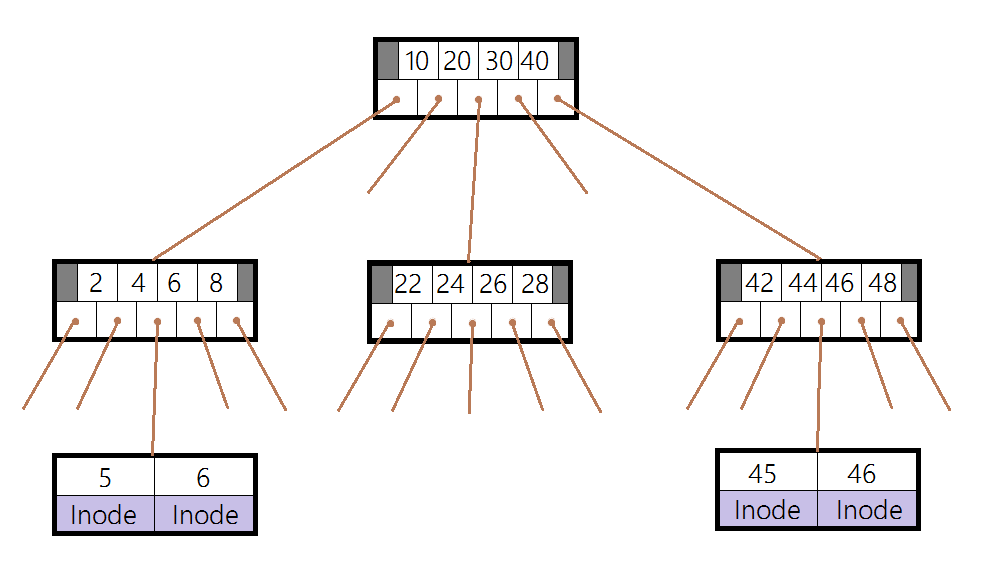
\includegraphics[width=\textwidth]{../images/btree.png}
	\end{figure}
\end{frame}

\begin{frame}{Difficulties}
	\begin{block}{Change in a file}
		\begin{itemize}
			\item[$\rightarrow$] changes location of files data
			\item[$\rightarrow$] changes location of Inode
			\item[$\rightarrow$]changes location of corresponding leave
			\item[$\rightarrow$]changes location of every parent branch including root node
		\end{itemize}
	\end{block}
	\begin{block}{How to approach}
		\begin{itemize}
			\item Reduce wear by caching a subset of tree index and root node address
			\item But still: how to find a ever changing root node?
		\end{itemize}
	\end{block}
\end{frame}


\begin{frame}{Tree Index}
	\begin{figure}[H]
		\centering
		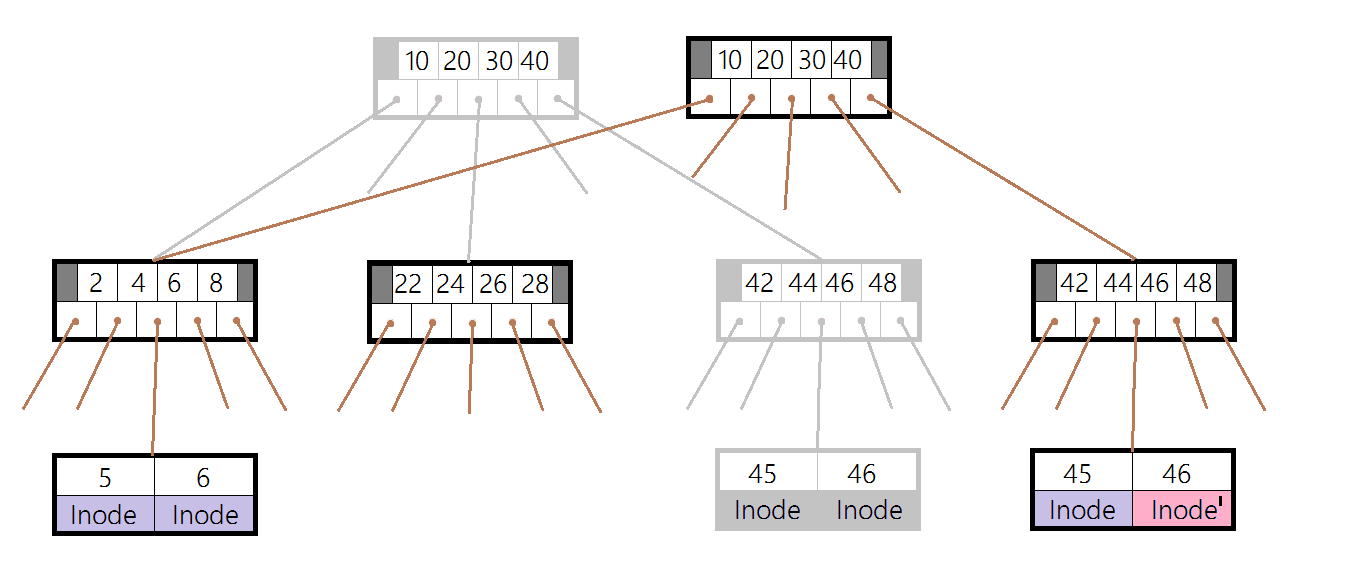
\includegraphics[width=\textwidth]{../images/btree_2.png}
	\end{figure}
\end{frame}

\subsection{Superblock}
\begin{frame}{Superblock}
	\begin{block}{Chaining}
		\begin{itemize}
			\item First two valid Areas contain anchor entries pointing to jump pads
			\item Jump pads point to other pads until final super page is reached
			\item Super page contains address of root node and uncommitted area summaries
		\end{itemize}
	\end{block}
\end{frame}

\subsection{Areas und Garbage Collection}
\begin{frame}{Areas}
	\begin{block}{}
		\begin{itemize}
			\item Combine erase blocks to a logical group
			\item Act as a single erase block
			\item Abstract logical and physical position on flash
			\item Contain only data of one type of \texttt{superblock}, \texttt{index}, \texttt{data} and \texttt{journal}
		\end{itemize}
	\end{block}
\end{frame}

\begin{frame}{Areas}
	\begin{figure}[H]
		\centering
		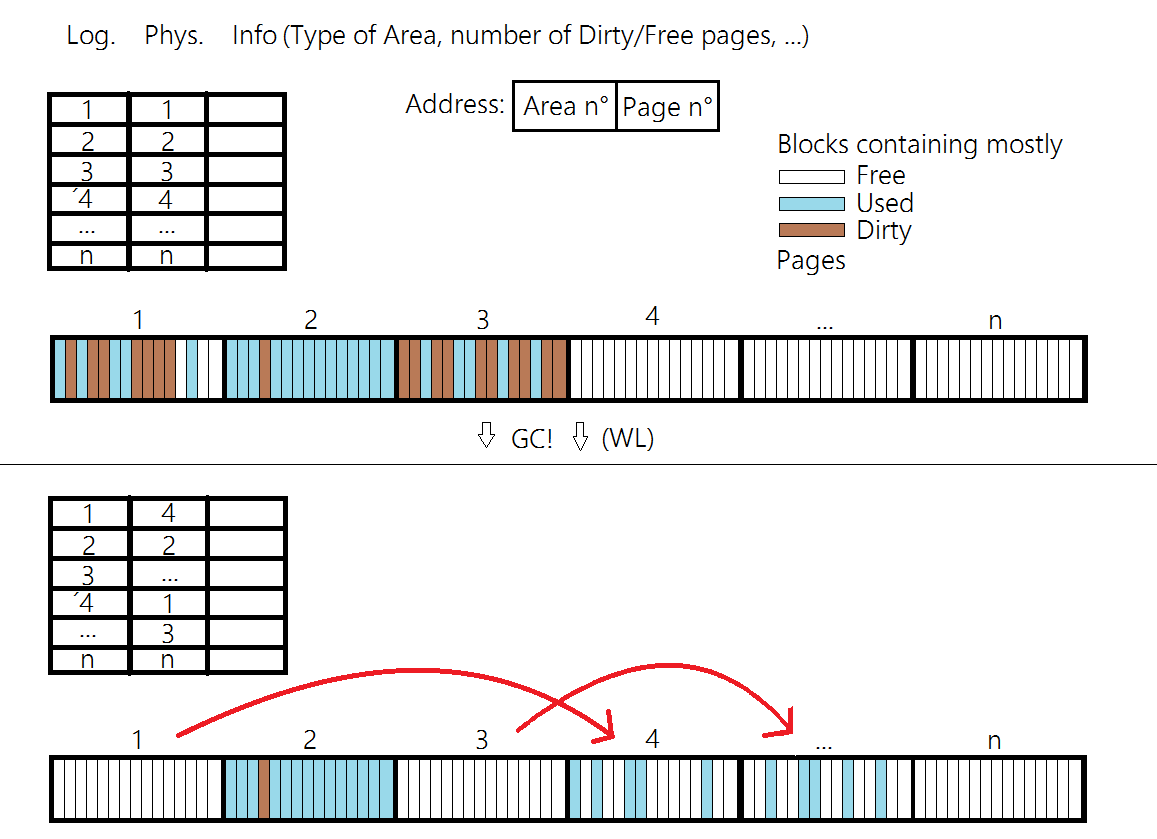
\includegraphics[height=0.9\textheight]{../images/Areas_address.png}
	\end{figure}
\end{frame}

\subsection{Fehlerkorrektur und Redundanz}
\begin{frame}{Fehlerkorrektur}
	\begin{block}{}
		\begin{itemize}
			\item a
		\end{itemize}
	\end{block}
\end{frame}
\end{document}